\section{Challenges of network machine learning}
\label{sec:ch1:challenges}

Like other branches of science, network machine learning is not without its challenges. There are infinitely many ways in which your network, or networks, that you actually get to analyze might have imperfections which can most efficiently be described as random. Rather than collecting data from every single person on the social network, or obtaining brain networks from every single person who could {potentially} be a musician, or collecting pristine data that always represents the underlying network perfectly, you instead look at a reasonably sized subset of data which you can feasibly obtain. Maybe this means collecting your social network with only $1000$ nodes instead of one hundred million, or maybe this means looking at $200$ brain networks instead of a network from every person in the United States.

In this book on network machine learning, we are going to focus some level of attention on the sub-branch of machine learning known as statistical learning. \textit{Statistical learning} is a framework for machine learning in which we {infer} things about our network by using statistics to refine and conceptualize our problem and quantify how reasonable our conclusions are. What exactly do we mean by this?

\subsubsection{We might imperfectly observe the network}

In many branches of science, collecting network data can be an imperfect and noisy process. It was only recently that we acquired a detailed map of the connectome of a complex organism, the fruit fly larva \cite{Winding2023Mar}. Even though fruit fly larvae are small, this is a substantial undertaking: their brain comprises several thousand neurons, and hundreds of thousands of edges, all fit into a volume smaller than cubic millimeter. In order to study the brain at the neuron-scale, the brain was sliced into thousands of tiny pieces smaller than a human hair, and each piece individually examined with a microscope. From there, extremely complicated algorithms and manual tracing were performed to stitch, slice-by-slice, which neurons connected with which neurons. To make this process even more difficult, everything was done on a single organism; with each step there was extremely minimal room for error. This neuron-by-neuron map was used to construct a network (called the \textit{connectome} of the organism) where the nodes were neurons and the edges were the neuron-to-neuron connections.

\begin{figure}[h]
    \centering
    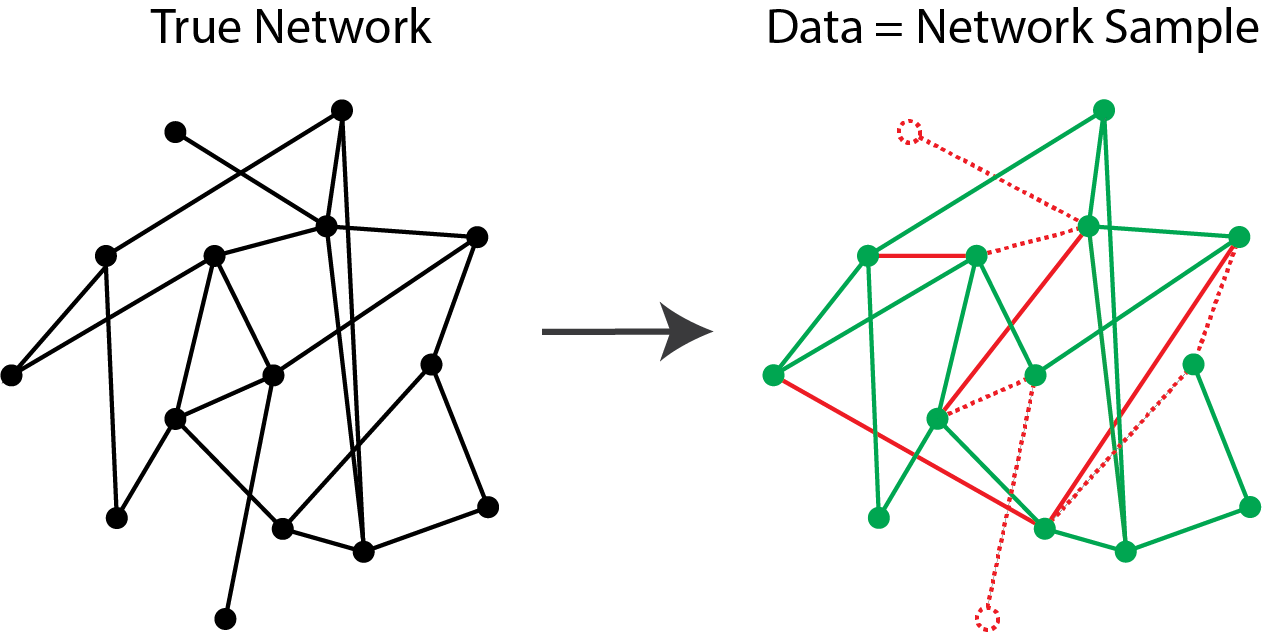
\includegraphics[width=0.7\linewidth]{foundations/ch1/Images/errorful_obs.png}
    \caption[Errorfully observe networks]{The true underlying network contains a lot of information that in the
course of observing or sampling the network, we don't actually measure properly. }
    \label{fig:ch1:errorful_net}
\end{figure}

With so many areas for potential error, it is almost impossible that the network is absolutely perfect. We might have missed some neurons, we might have missed some connections, and there might have been small mistakes anywhere in this complicated process. Figure \ref{fig:ch1:errorful_net} explores what it means for a network to be imperfectly observed. On the left, we see the true network we're trying to obtain. On the right, we see the actual network we obtained: we might be missing some of the nodes (red dashed nodes), we might be missing some of the edges (red dashed edges), or we might see edges which shouldn't really be present (red solid edges). While a portion of the network might faithfully represent the underlying system (green nodes and edges), we don't actually get to see what part of our sample is faithful or unfaithful with respect to the underlying network. The key is that when we attempt to build network machine learning systems, we need to be able to derive insights that are robust to these imperfect observations. This is because in some cases, it might be impossible to ever obtain the data that we need otherwise.

\subsubsection{We might not see the whole network}

When we study a network, it is rare that we observe the entire system perfectly in its entirety. For instance, a social network, in which the nodes of our network are people within the network, and edges are whether groups of people are friends with one another. If we wanted to study the network in its rawest form, we might need to collect data from millions, or billions, of accounts to construct a network that might take an infeasible amount of space just to store. Actually analyzing the network represents another huge hurdle; we would need to be able to devise techniques which could efficiently churn through terabytes worth of data. On the other hand, perhaps we could focus our attention on a subset of the network involving a few thousand or hundred thousand people. On this reduced subset of people, we might be much more free to ask rich questions, as we might not be nearly as limited in terms of the techniques that we can use on the data in a feasible time frame.

On a related note, the example that we gave for the fruit fly larva (drosophila) connectome was certainly not the first time connectomes have ever been investigated; people have been studying brain networks for decades. Before that paper came out, in fact, the drosophila larva has been a major focus of many connectome analyses. Due to the massive economic, computational, and anaytical challenges, however, earlier investigations focused on subsets of the brain, rather than on the whole thing. Despite only collecting bits and pieces of the network, major insights were learned which directly informed the effort to collect the entire network.

In both of these cases, you can learn a lot of valuable information by reducing the size of your network, learning from it, and then applying what you learned to the entire network. In Figure \ref{fig:ch1:nodes_ss}, we see an example where we only get to see a subset of the nodes in the network.

\begin{figure}[h]
    \centering
    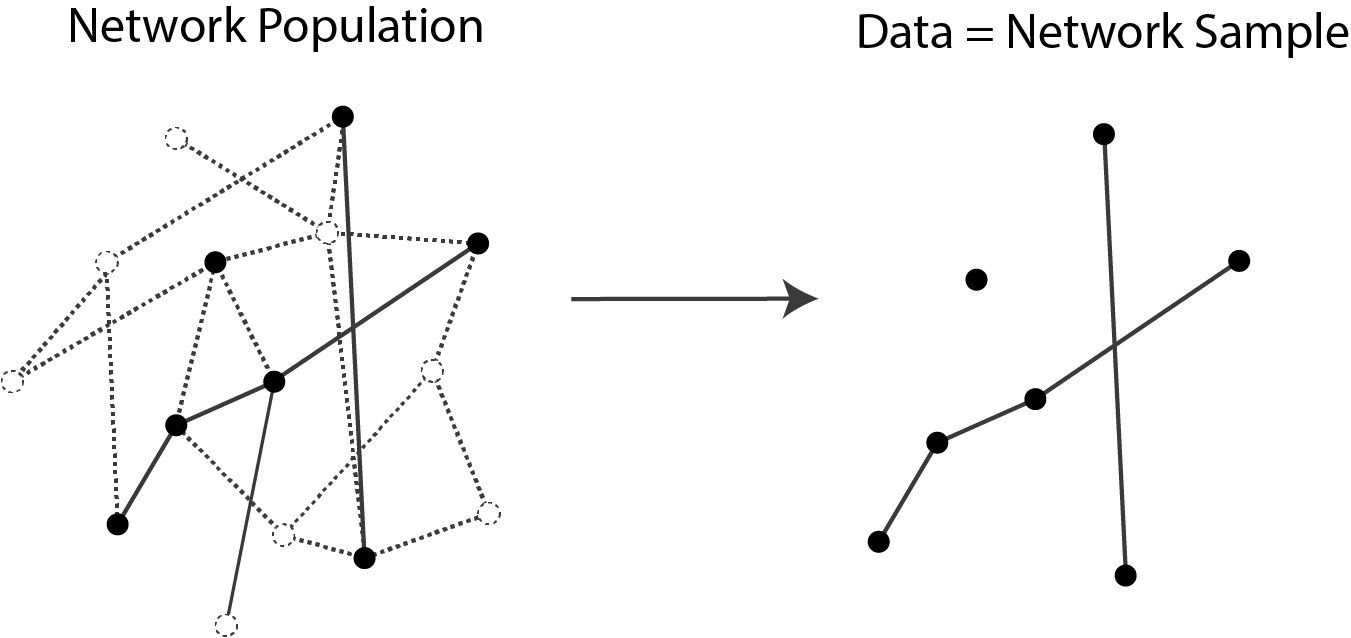
\includegraphics[width=0.8\linewidth]{foundations/ch1/Images/nodes.png}
    \caption[Only see subset of nodes]{The true underlying network has both solid and dashed edges and nodes, indicated in the left panel. However, when we sample the network on the right, our sample only includes the subset of nodes and edges that are solid.}
    \label{fig:ch1:nodes_ss}
\end{figure}


\subsubsection{We might only see a subset of the networks}

On a related note, let's put ourselves back in the mindset for the musician and non-musician brain networks from Example \ref{box:ch1:brainnet}. A team of psychologists might hypothesize that the brains of musicians tend to be much better connected in areas responsible for fine motor coordination and hearing, which are crucial skills for many instruments. To test this hypothesis, the psychologists could take one of two approaches. They could collect brain networks from every individual, or they could collect a subset of brain networks from groups of musicians and non-musicians in their area. In Figure \ref{fig:ch1:many_nets_ss}, we see an example where we only get to sample a subset of the networks in the underlying population. Despite the fact that the psychologists only studied a subset of musicians and non-musicians, with some statistical assumptions they can derive conclusions that will apply more broadly than just the group of people they analyzed.

\begin{figure}[h]
    \centering
    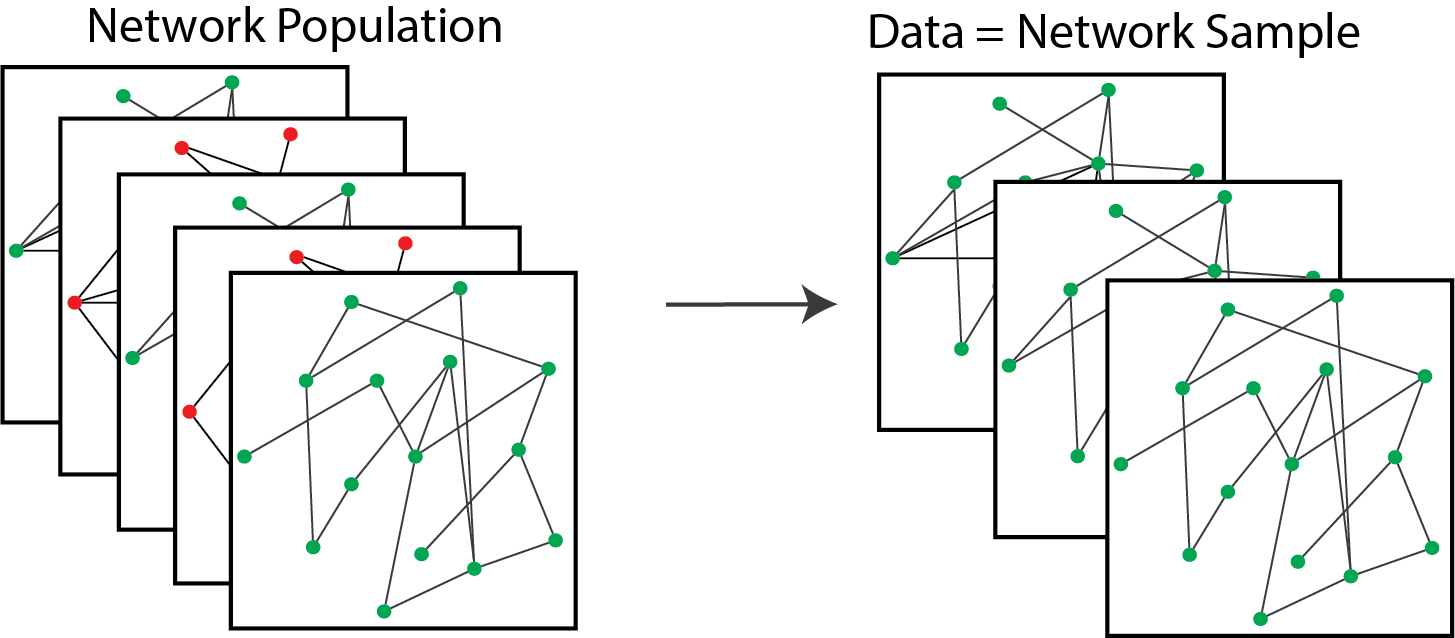
\includegraphics[width=0.7\linewidth]{foundations/ch1/Images/many_networks.png}
    \caption[Only see subset of networks]{The true underlying population contains many more networks than we are
able to actually sample. In the left panel, we have green and red
networks, but in the sample, we only get to see the green networks.}
    \label{fig:ch1:many_nets_ss}
\end{figure}

\subsubsection{Statistics allows us to bridge what we learn from what we see with what we didn't get to see}

In these cases, you have collected a \textit{sample}, which can be loosely defined as a subset of objects which is collected from the population in some way. The sample itself is where statistics comes into play. When you reach a conclusion, you do not want to reach a conclusion that only applies to the specific group of people, or the specific network, that you analyzed in your sample. Statistics allows you to be as specific as you can about how, exactly, conclusions that you reach on the sample apply to the general population. We summarize this idea in Figure \ref{fig:ch1:stat-learning}. Note that the network population may have a different interpretation depending on you specific network question, and might be populations of many networks, or populations of networks with some level of randomness or uncertainty as to how the network was obtained. Throughout this book, the sample itself, and how it relates to the underlying population, will always be in focus and should be at the forefront of your mind. 

\begin{figure}[h]
    \centering
    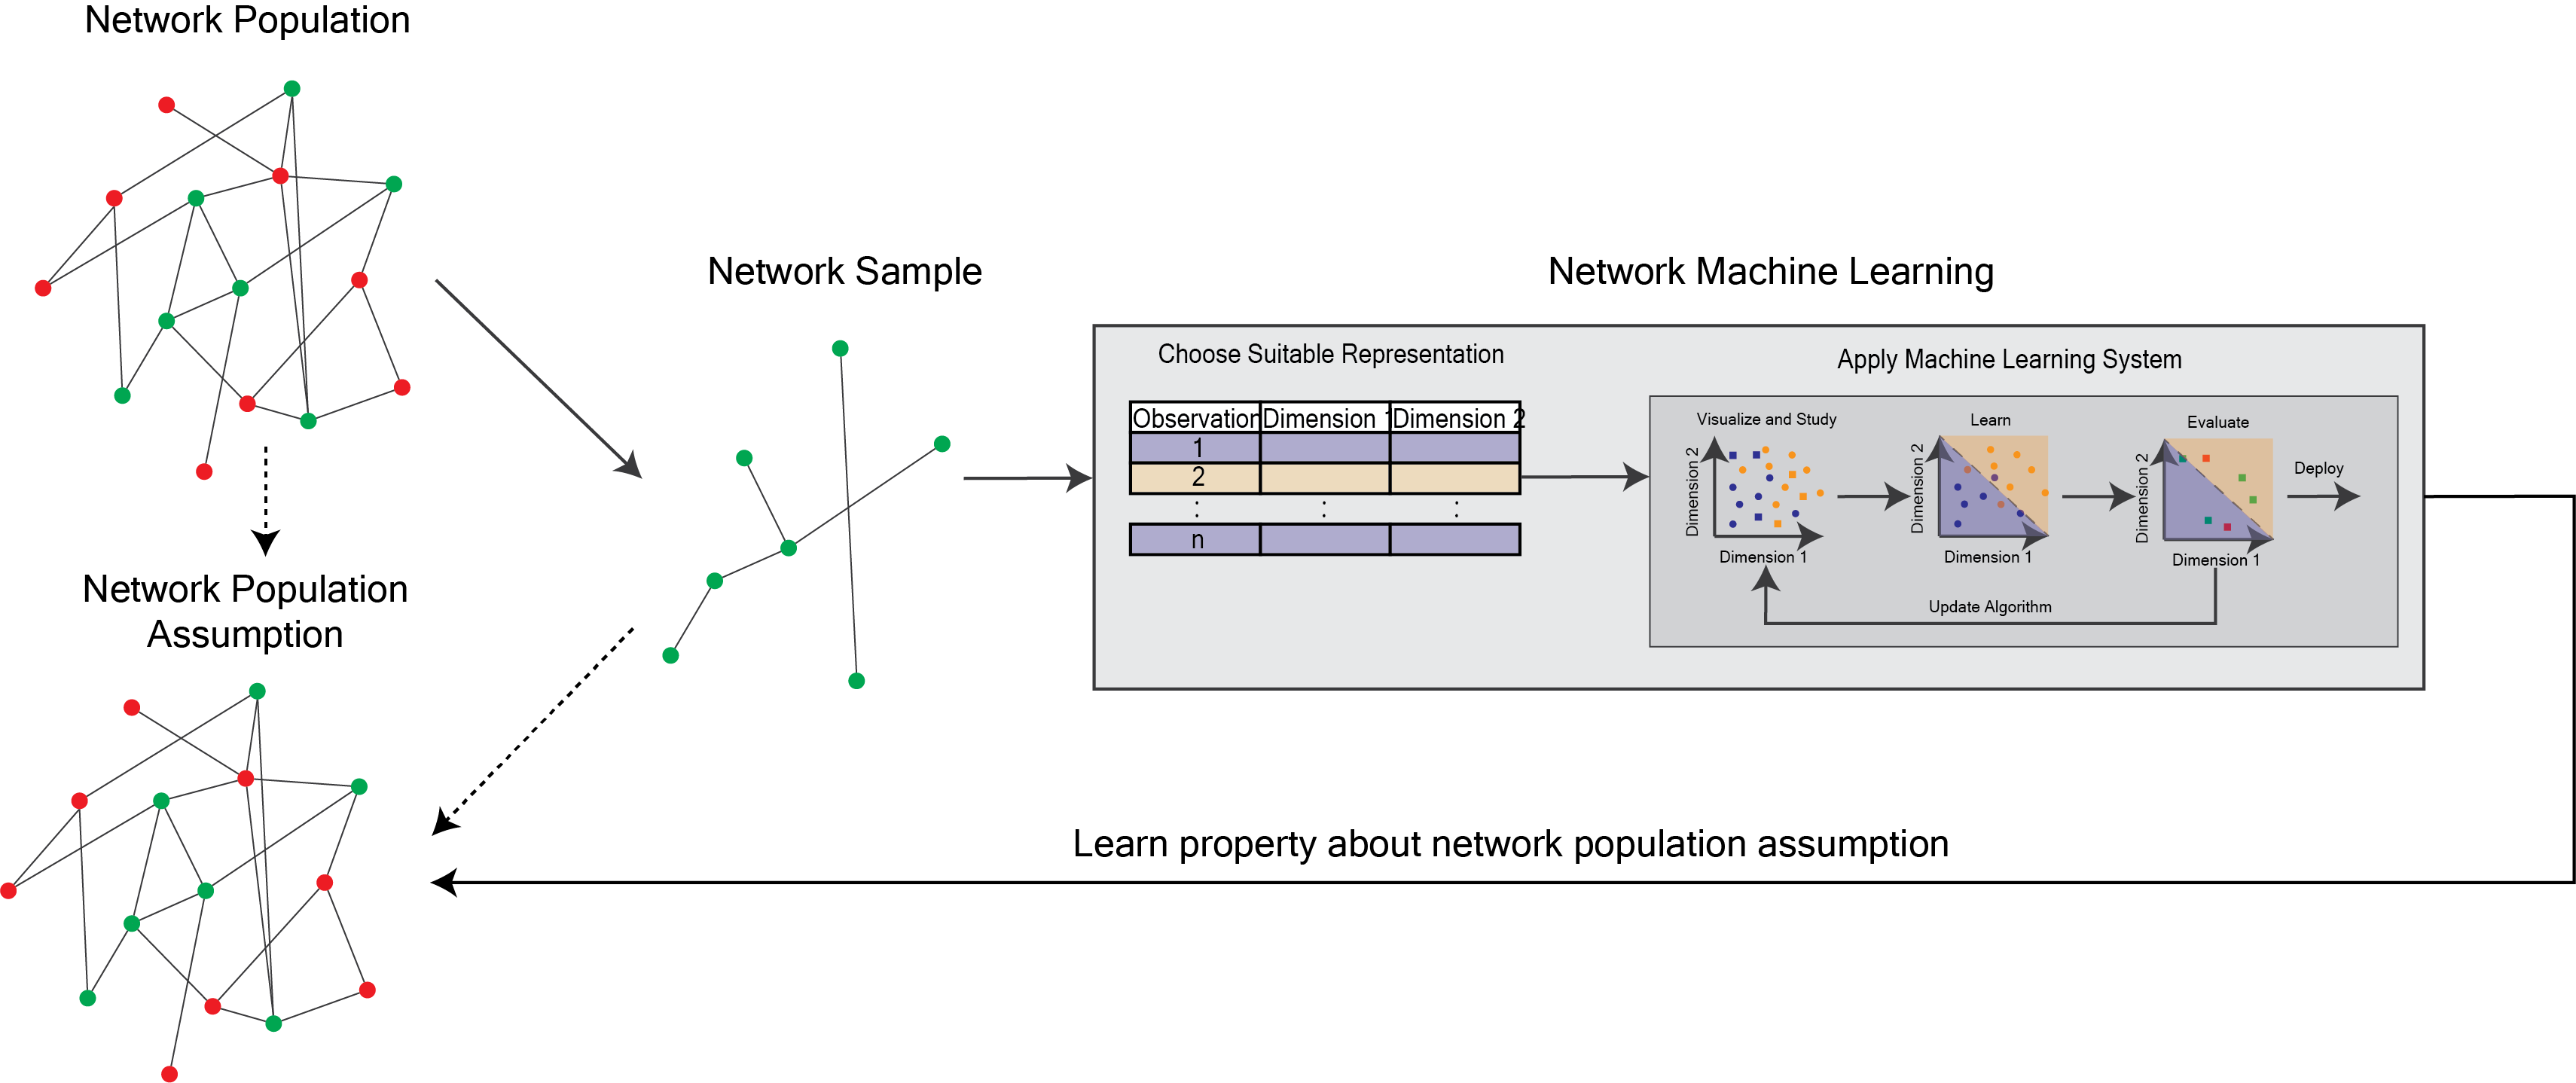
\includegraphics[width=\linewidth]{foundations/ch1/Images/apply.png}
    \caption[Statistical network machine learning]{We have a network population, which in this case, means a large network that we cannot properly observe. We obtain a sample of this network, and then use analyses on this sample and knowledge of how this sample was taken from the population to derive assumptions about our system. Ideally, this will faithfully represent the actual network population itself. Using network machine learning, we learn properties about the network population assumptions.}
    \label{fig:ch1:stat-learning}
\end{figure}


You {can} learn lots of valuable things about a sample without using statistics {at all}, and we will be sure to note when that is the case. However, if you want your conclusions to apply more broadly to the general population rather than the specific sample you collected, a reasonable way to do that quantitatively is using statistical learning.

\subsection{There are a variety of other challenges too!}

In Section \ref{sec:ch1:types}, you learned about some of the different types of network machine learning problems that we can start to address. Network machine learning is in its infancy, and these types of problems are constantly evolving. Deciding which group of categories your problem falls into, reshaping your question of interest to fit into problems that can be answered with existing techniques, the types of strategies that are at your disposal to answer your questions, or whether you need to develop new techniques all together to answer your question take lots of energy (and resources!). In the next few chapters, you'll see what example data analyses look like in network machine learning, which will hopefully give you a better idea of how these analyses are performed.

\newpage